% Informe del proyecto final — IA para investigación (FCEN-UBA, 2026)
% Compilar:  ./build.sh   (figuras + dos pasadas de pdflatex)
% v2: incorpora la revisión adversarial REVIEW_v1.md (61 observaciones).
\documentclass[11pt,a4paper]{article}
\usepackage[utf8]{inputenc}
\usepackage[T1]{fontenc}
\usepackage[spanish,es-noshorthands]{babel}
\usepackage{lmodern}
\usepackage[margin=2.4cm]{geometry}
\usepackage{graphicx}
\usepackage{booktabs,tabularx,longtable,array}
\usepackage{amsmath}
\usepackage{xcolor}
\usepackage[hidelinks]{hyperref}
\usepackage{caption}
\usepackage{enumitem}
\setlist{itemsep=2pt,topsep=3pt}
\graphicspath{{../figures/}}
\definecolor{nota}{HTML}{52514E}
\newcommand{\ev}[1]{{\small\color{nota}[#1]}}   % puntero a evidencia
\newcommand{\code}[1]{\texttt{#1}}

\title{\textbf{Una inversión que no era física}\\[4pt]
\large Estudio de caso de una investigación asistida por agentes de IA:\\
asimetrías azimutales de muones con el UMD del Observatorio Pierre Auger}
\author{Lautaro Silva Pizzi \and Manuel Racca\\[2pt]
{\small Proyecto final --- \emph{Investigación asistida por inteligencia artificial:}}\\
{\small \emph{aplicación en ondas gravitacionales} (Zaldarriaga), FCEN-UBA}}
\date{Septiembre de 2026}

\begin{document}
\maketitle

\begin{abstract}
\noindent
Reconstruimos, a partir de evidencia primaria (149 \emph{commits}, 49 transcripciones de sesiones de
Claude Code y Codex y los documentos que produjeron), cómo se investigó con agentes de IA una anomalía
de la tesis de licenciatura de L.~Silva Pizzi. En simulaciones Monte Carlo (protones, SIBYLL~2.3e,
$30^\circ$--$40^\circ$ de cenit), la amplitud del primer armónico azimutal $A_1$ del número de muones que
atraviesan los tanques del detector de superficie (SD) de Auger cambia de signo a grandes distancias del
núcleo, mientras que la del detector subterráneo de muones (UMD) no lo hace. Durante casi dos semanas, el
tesista y los agentes buscaron una explicación fenomenológica. La respuesta resultó ser un \emph{sesgo de
selección}: el observable del SD se construía sólo con estaciones presentes en el evento SD reconstruido.
Incluyendo todas las estaciones simuladas, la inversión desaparece en la muestra estudiada
($A_1=+0.069$ en lugar de $-0.124$ a 1200--1350\,m). El hallazgo central de este estudio es que
\emph{un subagente propuso la hipótesis correcta tres días antes de que se confirmara, pero fue
descartada con un test que no podía ponerla a prueba}. La rescató una lectura independiente: otro modelo,
con otro contexto, rechazó la premisa que había heredado. Discutimos qué prácticas funcionaron (memoria de
proyecto, revisión cruzada entre modelos, controles humanos), qué fallas aparecieron (verificaciones que no
lo eran, resúmenes que pierden información, código presentado sin ejecutar, errores silenciosos) y qué
recomendaciones se desprenden para físicos que trabajen con agentes.
\end{abstract}

\tableofcontents
\newpage

%=====================================================================
\section{Introducción}
%=====================================================================
El curso propuso usar agentes de IA «como asistentes para la investigación científica». Elegimos como caso
un problema real y, en su momento, abierto: la tesis de licenciatura de uno de nosotros (L.~Silva Pizzi,
ITeDA/FCEN-UBA; en adelante, «el tesista»). Su repositorio registra con inusual detalle cómo se trabajó con
los agentes. El período estudiado arranca con el curso: la primera sesión de Claude Code en el repositorio
es del 29/08/2026, el día siguiente a la clase «Primeros pasos con Claude Code» \ev{transcripción
\code{630c3828}; cronograma del curso}.

La pregunta que guía el estudio es concreta: \textbf{¿los agentes ayudaron o entorpecieron el
descubrimiento de que un efecto aparentemente físico era un artefacto de selección?} No usamos la memoria
de los participantes como fuente principal. Usamos los registros: \emph{commits}, transcripciones completas
de las sesiones y los documentos generados. Cuando la evidencia falta o es ambigua, lo decimos. Las citas
de mensajes originalmente en inglés están traducidas por nosotros.

%=====================================================================
\section{Contexto científico}
%=====================================================================
Un rayo cósmico de ultra alta energía que llega a la atmósfera produce una lluvia atmosférica extensa. El
Observatorio Pierre Auger la muestrea en el suelo con dos tipos de detector:
\begin{itemize}
  \item tanques Cherenkov de agua (SD), sensibles a la componente electromagnética y a muones de casi
  cualquier energía;
  \item en el arreglo de relleno (\emph{Infill}), centelladores enterrados a $\sim 2.3$\,m (UMD/AMIGA), que
  sólo registran muones por encima de $\sim 1\,\mathrm{GeV}/\cos\theta$.
\end{itemize}

En lluvias inclinadas, la densidad de partículas en el plano de la lluvia no es azimutalmente simétrica. La
región «temprana», la que el frente alcanza primero, y la «tardía» difieren por atenuación (dominante para
la componente electromagnética), por efectos geométricos (más relevantes para los muones) y, en menor
medida, por el campo geomagnético. Se parametriza
\begin{equation}
  \rho(\varphi) = \rho_0\,\bigl(1 + A_1\cos\varphi\bigr),
\end{equation}
con $\varphi$ medido en el plano de la lluvia desde la dirección temprana, de modo que $A_1>0$ indica un
exceso temprano. La tesis estudia $A_1$ con muones del UMD (según su planteo, por primera vez); por ahora,
sólo en simulaciones.

\paragraph{La anomalía.} En simulaciones Monte Carlo (CORSIKA + Offline; protones, SIBYLL~2.3e,
$30^\circ\!\le\theta<40^\circ$), el número de muones que atraviesan los tanques SD tiene $A_1>0$ cerca del
núcleo, pero \emph{cambia de signo} por encima de $\sim 950$\,m. El UMD, en cambio, se mantiene positivo
(figura~\ref{fig:anomalia}). La nota interna GAP-2026-041 \cite{gap041} presentó la inversión como «un
rasgo genuino» de la señal del SD y propuso dos mecanismos: uno cinemático (muones blandos y divergentes)
y uno instrumental (las paredes laterales del tanque). Según el tesista, una versión previa de la nota
contenía un argumento de «divergencia cinemática» que se retiró a pedido de su director.

\begin{figure}[t]
  \centering
  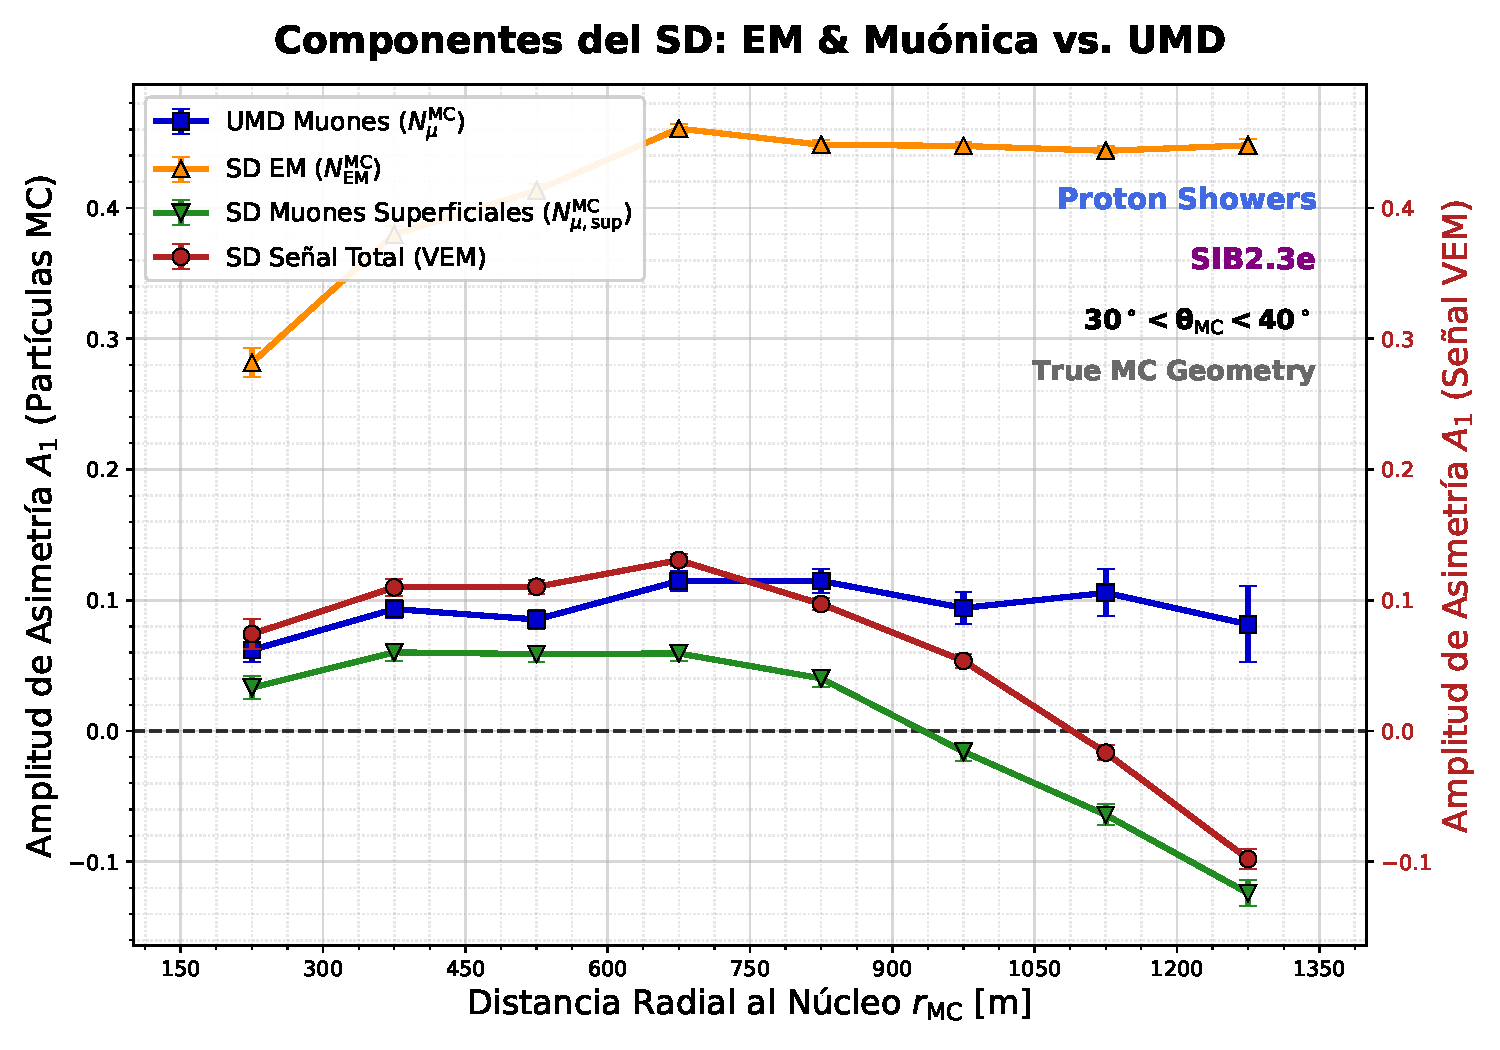
\includegraphics[width=0.78\linewidth]{sd_desglose_componentes_vs_umd.pdf}
  \caption{La anomalía tal como figuraba en la tesis: $A_1$ en función de la distancia al núcleo para el UMD
  (azul), la componente muónica del SD (verde), la electromagnética (naranja) y la señal total (rojo). La
  curva verde se vuelve negativa por encima de $\sim 950$\,m. Todas las curvas incluyen, sin indicarlo, el
  requisito de estación SD reconstruida. Figura de la tesis (\code{Scripts/plots\_seccion\_6.py}),
  reutilizada.}
  \label{fig:anomalia}
\end{figure}

%=====================================================================
\section{Cómo hicimos esta reconstrucción}
%=====================================================================
El estudio es, a su vez, un ejercicio con agentes. Las fuentes fueron:
\begin{itemize}
  \item el historial de \code{git}: 149 \emph{commits} (122 sin contar fusiones) y 23 \emph{pull requests}
  desde el 29/08;
  \item 49 transcripciones locales, convertidas a texto legible con un script propio:
  \begin{itemize}
    \item 20 sesiones principales de Claude Code (dos vacías, más la de este estudio);
    \item 16 transcripciones de sus subagentes;
    \item 13 de Codex: 4 sesiones de trabajo, 3 subagentes y 6 hilos del revisor automático de acciones;
  \end{itemize}
  \item los documentos generados por los agentes en \code{claude\_work/}, el cuaderno de laboratorio de la
  tesis y los capítulos 3, 5 y 6.
\end{itemize}
Una sesión coordinadora de Claude (Opus~5.5) repartió la lectura entre ocho agentes paralelos, uno por
familia de fuentes. Todos tenían una consigna común: cada afirmación lleva su evidencia (hash de
\emph{commit}, \code{archivo:línea} o \code{sesión @ hora}) y lo no verificado se marca como tal. Un noveno
agente verificó contra las fuentes primarias 21 afirmaciones clave; confirmó 20 y matizó una. Un décimo
revisó este informe en modo adversarial. El proceso tuvo sus propias fallas, que documentamos en el
apéndice~\ref{ap:metodo}.

%=====================================================================
\section{Cronología}
%=====================================================================
La figura~\ref{fig:timeline} resume el período 28/08--24/09/2026 (desde el inicio del curso) y el apéndice~\ref{ap:crono} lo detalla.
Distinguimos cinco etapas.

\begin{figure}[t]
  \centering
  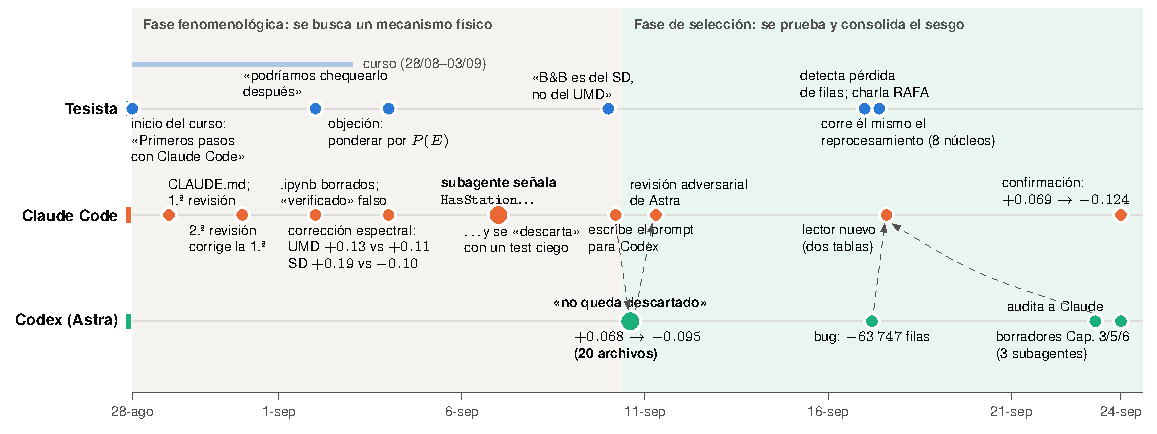
\includegraphics[width=\linewidth]{timeline.pdf}
  \caption{Línea de tiempo del proceso, por actor. Los puntos grandes marcan los dos momentos en que apareció
  la hipótesis de selección. Las flechas punteadas indican revisión cruzada entre modelos. Elaboración
  propia a partir de \code{timeline.md}.}
  \label{fig:timeline}
\end{figure}

\subsection{Antes de los agentes (sep.\ 2025 -- ago.\ 2026)}
Durante un año, el tesista construyó con sus directores el pipeline ADST$\to$parquet$\to$ajuste de $A_1$,
sin agentes de IA. Según el tesista, en esa etapa sólo usó Gemini como chatbot web, sin agentes de
programación; algunos comentarios del código de noviembre de 2025 tienen el estilo de esas respuestas, pero no
sabemos si algún cambio concreto salió de allí. En esa etapa encontró y corrigió
errores reales. Uno de ellos, una doble resta del azimut en el Anillo Denso, había producido «inversiones»
dependientes de la masa que el propio tesista retiró como un «error de pipeline, no de física»
\ev{\code{Trabajo.tex:470}; \code{ce4e0eb}}. También descartó sospechas infundadas sobre Offline
\ev{\code{b0f562d}}.

En octubre de 2025 entró al lector de simulaciones la línea
\begin{center}
\code{sdStation = sEvent.GetStationById(sdId) if sEvent.HasStation(sdId) else None}
\end{center}
al principio, como simple protección contra punteros nulos \ev{\code{e9a2737}}. El 5/11 pasó a descartar
la fila entera cuando no hay estación SD reconstruida («sin sdStation no hay geometría»). El 11/11 quedó
rotulada «Corte de Calidad 1: Geometría» \ev{\code{41b98be}, \code{ce4e0eb}; hoy
\code{Procesamiento\_ADST\_v8-2.py:182--187}}.

El lector, además, recorre los contadores del UMD, y Offline no escribe módulos UMD para estaciones SD sin
disparo. La selección estaba, por lo tanto, en la \emph{definición de la población}; la línea sólo la hacía
explícita. El motivo del corte era razonable: si el SD no dispara, el UMD no guarda datos, y esas filas
parecían inútiles. Ninguna nota, capítulo ni versión de la nota GAP menciona la selección de estaciones. En julio
de 2026, el tesista abandonó un modelo Monte Carlo rápido con el que intentaba explicar la inversión
\ev{\code{6d6b97b}}.

\subsection{Incorporación de agentes y primeras revisiones (28/08--02/09)}
\begin{itemize}
  \item \textbf{29/08: \code{CLAUDE.md}.} Claude (Sonnet~5) construyó \code{CLAUDE.md}, un archivo de
  contexto del proyecto, apoyándose en tres subagentes de exploración lanzados en paralelo. Lo subió al
  repositorio sin que se lo pidieran. En la hora siguiente, el tesista lo corrigió tres veces:
  \begin{itemize}
    \item un supuesto «bug confirmado» de Offline, tomado de notas viejas, que él ya había descartado;
    \item la política de \code{git};
    \item la equivalencia del título \ev{\code{fa012d6}$\to$\code{db90346}}.
  \end{itemize}
  \item \textbf{29/08: primera revisión.} La escribió Sonnet~5 y no Opus, como pretendía el tesista: el
  \code{/model opus} escrito dentro del prompt no tuvo efecto. Concluyó que retirar el argumento de
  divergencia cinemática estaba justificado y que la nota publicada estaba «bien argumentada»
  \ev{\code{c468bc17}}.
  \item \textbf{31/08: segunda revisión.} Opus~5 recibió la consigna de «construir sobre lo previo, pero
  reverificarlo» y corrigió la primera revisión: las razones estaban mal ordenadas y el argumento
  instrumental de la nota tenía el signo equivocado \ev{\code{df3c0277}}.
\end{itemize}

El 2/09, sin un mecanismo convincente, el tesista escribió: \emph{«los datos que analicé no parecen tener
errores ni bugs (podríamos chequearlo después), así que [\ldots] la inversión de signo en el SD y no en el
UMD es física. Se ve tanto en el Anillo Denso como en el Infill, con coordenadas MC y REC»}
\ev{\code{df3c0277} @ 14:26 UTC}. La auditoría del pipeline quedó postergada.

\subsection{La fase fenomenológica (03/09--10/09)}
Los agentes exploraron sucesivamente:
\begin{itemize}
  \item la divergencia cinemática \cite{cazon};
  \item la geometría del tanque;
  \item la dispersión coulombiana en vuelo;
  \item la dependencia de la densidad muónica con la profundidad.
\end{itemize}
Dos momentos son especialmente instructivos:
\begin{itemize}
  \item \textbf{Una objeción del tesista corrige un error.} El tesista señaló que el cálculo ponderado por
  espectro no pesaba cada ángulo por su probabilidad a esa energía. Opus~5 confirmó el error y lo localizó:
  un promedio de cocientes en lugar de un cociente de integrales, que venía de una pasada anterior de
  Sonnet. Con el cálculo corregido, el modelo predice $+0.13$ para el UMD (frente a un $+0.11$ observado,
  aunque la coincidencia depende del estimador y del binado) y $+0.19$ para el SD (observado: $-0.10$)
  \ev{\code{67ae9e4}}. \emph{El modelo parecía funcionar para un detector y fallaba sólo para el otro.}
  Ese mismo día, Opus planteó por escrito si el conteo muónico del SD «arrastra una selección a nivel de
  detector».
  \item \textbf{Una objeción del tesista fuerza una retractación.} Un agente propuso trasladar al UMD un
  resultado de Bertou y Billoir \cite{bb} obtenido para el SD. El tesista objetó que el SD tiene mucha más
  masa interactuante. El agente agregó la diferencia de umbral, se retractó de la propuesta, la dejó
  documentada como callejón sin salida y la guardó como lección permanente en su memoria
  \ev{\code{88fffbb}}.
\end{itemize}

\paragraph{El casi-hallazgo del 7/09.} Esa sesión recibió una consigna binaria, surgida de la dirección de
la tesis: explicar matemáticamente la diferencia SD/UMD o recortar la derivación. Al plantear el trabajo,
Opus~5 decidió por iniciativa propia revisar «algo que las pasadas previas nunca examinaron: cómo entran las
estaciones a la muestra». Todavía no había leído el documento del 4/09. Un subagente respondió en cuatro
minutos:
\begin{quote}
\emph{«Este \code{sEvent.HasStation(sdId)} en la línea 182 es la única compuerta de disparo/selección, sin
etiquetar, de todo el pipeline [\ldots]. Si [el evento SD] contiene sólo estaciones con disparo, entonces a
grandes $r$ la región tardía pierde estaciones preferentemente y las que sobreviven están fluctuadas hacia
arriba»} \ev{subagente \code{a7da6dcd} @ 14:12 UTC}.
\end{quote}
La ejecución (Sonnet~5, sobre el plan de Opus) midió que la \emph{cantidad} de estaciones por bin de azimut
estaba fuertemente modulada y correlacionada con $A_1^{\mathrm{SD},\mu}$ ($r=-0.89$). El informe llegó a
registrarlo como «exactamente el patrón que haría sospechar a un árbitro». Luego aplicó un \emph{bootstrap}
que igualaba el número de filas por bin, vio que $A_1$ no cambiaba ($-0.0945\to-0.0943$) y concluyó que la
hipótesis «no sobrevive a la prueba directa» \ev{\code{60fca507} @ 14:23}. El informe resultante no
menciona \code{HasStation} y recomienda presentar la inversión como «un resultado MC robusto, que se mostró
que no es un artefacto del pipeline» \ev{\code{unified\_asymmetry\_model\_v1/report.md}}.

El test sí descartaba que el número desigual de filas sesgara el ajuste. Lo que no podía detectar era lo que
se buscaba. Submuestrear al azar las filas que \emph{sobrevivieron} no cambia la media condicional de cada
bin. El sesgo estaba en \emph{cuáles} estaciones sobreviven, y las eliminadas no estaban en el archivo por
construcción.

\subsection{Astra y el sesgo de selección (10/09--11/09)}
El 10/09, el tesista pidió a Claude (Sonnet~5) que redactara un prompt para Codex (modelo
\code{gpt-6-astra}, «Astra») con el fin de hacer una revisión «con máxima potencia». La elección fue
deliberada: Astra se presentaba públicamente como un modelo de punta, y el tesista quería ver cómo se
comportaban modelos de distintas empresas frente al mismo problema. El prompt se pegó sin
cambios: una copia idéntica de 14\,688 caracteres. Pedía buscar una posible «selección a nivel de detector»
en el conteo muónico, pero no mencionaba \code{HasStation} y sostenía que la auditoría de muestreo «debe
tratarse como establecida» \ev{\code{60fca507} @ 14:06; Codex \code{01a08ba1} @ 14:10}. Doce minutos
después de empezar, tras leer el código fuente de Offline y el lector de la tesis, Astra escribió:
\begin{quote}
\emph{«Hay otra selección que sí merece comprobarse: el parquet exige una estación SD reconstruida para
conservar la fila UMD. Eso no queda descartado por el bootstrap anterior, que sólo comprobó el efecto de
tener distinto número de filas por bin.»} \ev{Codex \code{01a08ba1} @ 14:22 UTC}
\end{quote}
Esa misma tarde, con una interrupción de cuatro horas por límite de uso, leyó los archivos ADST con un lector
propio y simplificado, no con el pipeline del tesista. Eso lo aclaró recién cuando el tesista se lo preguntó.
Resultados, con 20 archivos y 106\,280 pares estación--evento en la banda 1050--1400\,m:
\begin{itemize}
  \item $A_1=+0.068$ con todas las estaciones simuladas;
  \item $A_1=-0.095$ exigiendo estación reconstruida, idéntico al parquet original fila a fila;
  \item diferencia pareada $-0.162$, IC\,95\,\% $[-0.178,-0.145]$, con \emph{bootstrap} agrupado por lluvia
  CORSIKA original \ev{\code{01a08ba1} @ 19:30}.
\end{itemize}
Al día siguiente, Astra reprodujo la figura del tesista (con diferencias de hasta $\sim10^{-9}$) antes de
agregarle la curva sin corte. En sus informes separó lo demostrado (el efecto de la selección) de lo
hipotético (el mecanismo). También rechazó la lectura exagerada del propio tesista, «la razón de la
asimetría es entonces un sesgo del detector»: no se había demostrado un error de Offline.

Sobre el método fue menos precisa. Cuando el tesista preguntó si había usado «literalmente» su código salvo
esa línea, respondió: \emph{«No, no literalmente. [\ldots] Mi redacción anterior debió dejarlo más claro»}
\ev{\code{01a08ba1} @ 16:53 del 11/09}. Esa pregunta del tesista motivó el reprocesamiento sobre su propio
pipeline.

\subsection{Revisión cruzada y consolidación (11/09--24/09)}
A partir de allí, los dos modelos se revisaron mutuamente (figura~\ref{fig:workflow}):
\begin{itemize}
  \item \textbf{Claude revisa a Astra (11/09).} La revisión escéptica, planificada por Opus~5 y ejecutada por
  Sonnet~5, usó seis subagentes de revisión y uno adversarial. Veredicto: «parcialmente de acuerdo». El
  efecto es real y está bien medido; el mecanismo no está demostrado; la validez se limita a
  $30$--$40^\circ$, protones y un modelo hadrónico.
  \item \textbf{Código presentado sin ejecutar (11/09--17/09).} Astra entregó dos lectores «preparados, no
  ejecutados» sobre datos reales. En el segundo, pensado como un cambio «mínimo», introdujo la condición
  \code{or not simCounter} y la describió como «protección inofensiva»; una de sus pruebas sintéticas la
  daba por buena. Al correrlo, el tesista notó que \emph{el número de filas bajó}. Astra reconoció la pérdida
  (63\,747 filas) y el cambio \ev{\code{01a08ba1}, 17/09}. Además, marcar la línea como bandera no
  alcanzaba: sin estación SD con disparo tampoco hay módulo UMD, así que el $A_1$ del SD daba $-0.110$ con y
  sin bandera.
  \item \textbf{Claude corrige el diseño (17/09)} con un lector que recorre por separado las estaciones
  simuladas, y lo valida fila a fila contra el parquet original. El tesista corre él mismo el
  reprocesamiento completo, en ocho núcleos del servidor compartido \ev{\code{8d4b5a0}, \code{0ecae20}}.
  \item \textbf{Astra audita a Claude (23/09).} Verifica sobre el parquet reprocesado los números de Claude y
  encuentra tres huecos en sus validaciones.
\end{itemize}

La figura~\ref{fig:resolucion} muestra el resultado sobre el pipeline del tesista. Sin el requisito, el SD
muónico queda positivo: $+0.069$ a 1200--1350\,m, frente a $-0.124$ con él \ev{\code{c332ab8}}. Queda
estadísticamente compatible con el UMD en los tres bines lejanos, aunque sistemáticamente por debajo en todo
el rango, y la diferencia es significativa entre 150 y 900\,m.

Hay que aclarar que el UMD también está restringido a estaciones con disparo del SD, y su $A_1$ no se puede
«des-seleccionar» con estos archivos. Que siga positivo sugiere que el conteo del UMD, hecho por otro
detector y con otro umbral, está mucho menos correlacionado con el disparo del SD que el propio conteo del
tanque. Mecanismo propuesto, todavía como hipótesis: a grandes $r$ la probabilidad de conservar una estación
es baja, y menor del lado tardío (retención $\sim$52\,\% temprana contra $\sim$24\,\% tardía). Las estaciones
tardías que sobreviven lo hacen preferentemente por fluctuaciones hacia arriba de su señal, incluida la
muónica.

La charla del tesista en RAFA 2026 (17/09) mostró el resultado de Astra como «análisis preliminar», antes de
este reprocesamiento. Según el tesista, su director se sorprendió pero lo encontró creíble, y la dirección
aprobó el resultado. También pidió un control adicional, todavía pendiente: verificar si la mayoría de las
estaciones que elimina el requisito tenían un solo muón atravesándolas. Si tuvieran más, sería extraño que
no hubieran disparado. El traspaso del reprocesamiento de Astra a Claude (17/09) se debió al límite de uso
de Codex. Los borradores de los capítulos 3, 5 y 6 que incorporan el resultado existen, pero todavía no
entraron al texto de la tesis.

\begin{figure}[t]
  \centering
  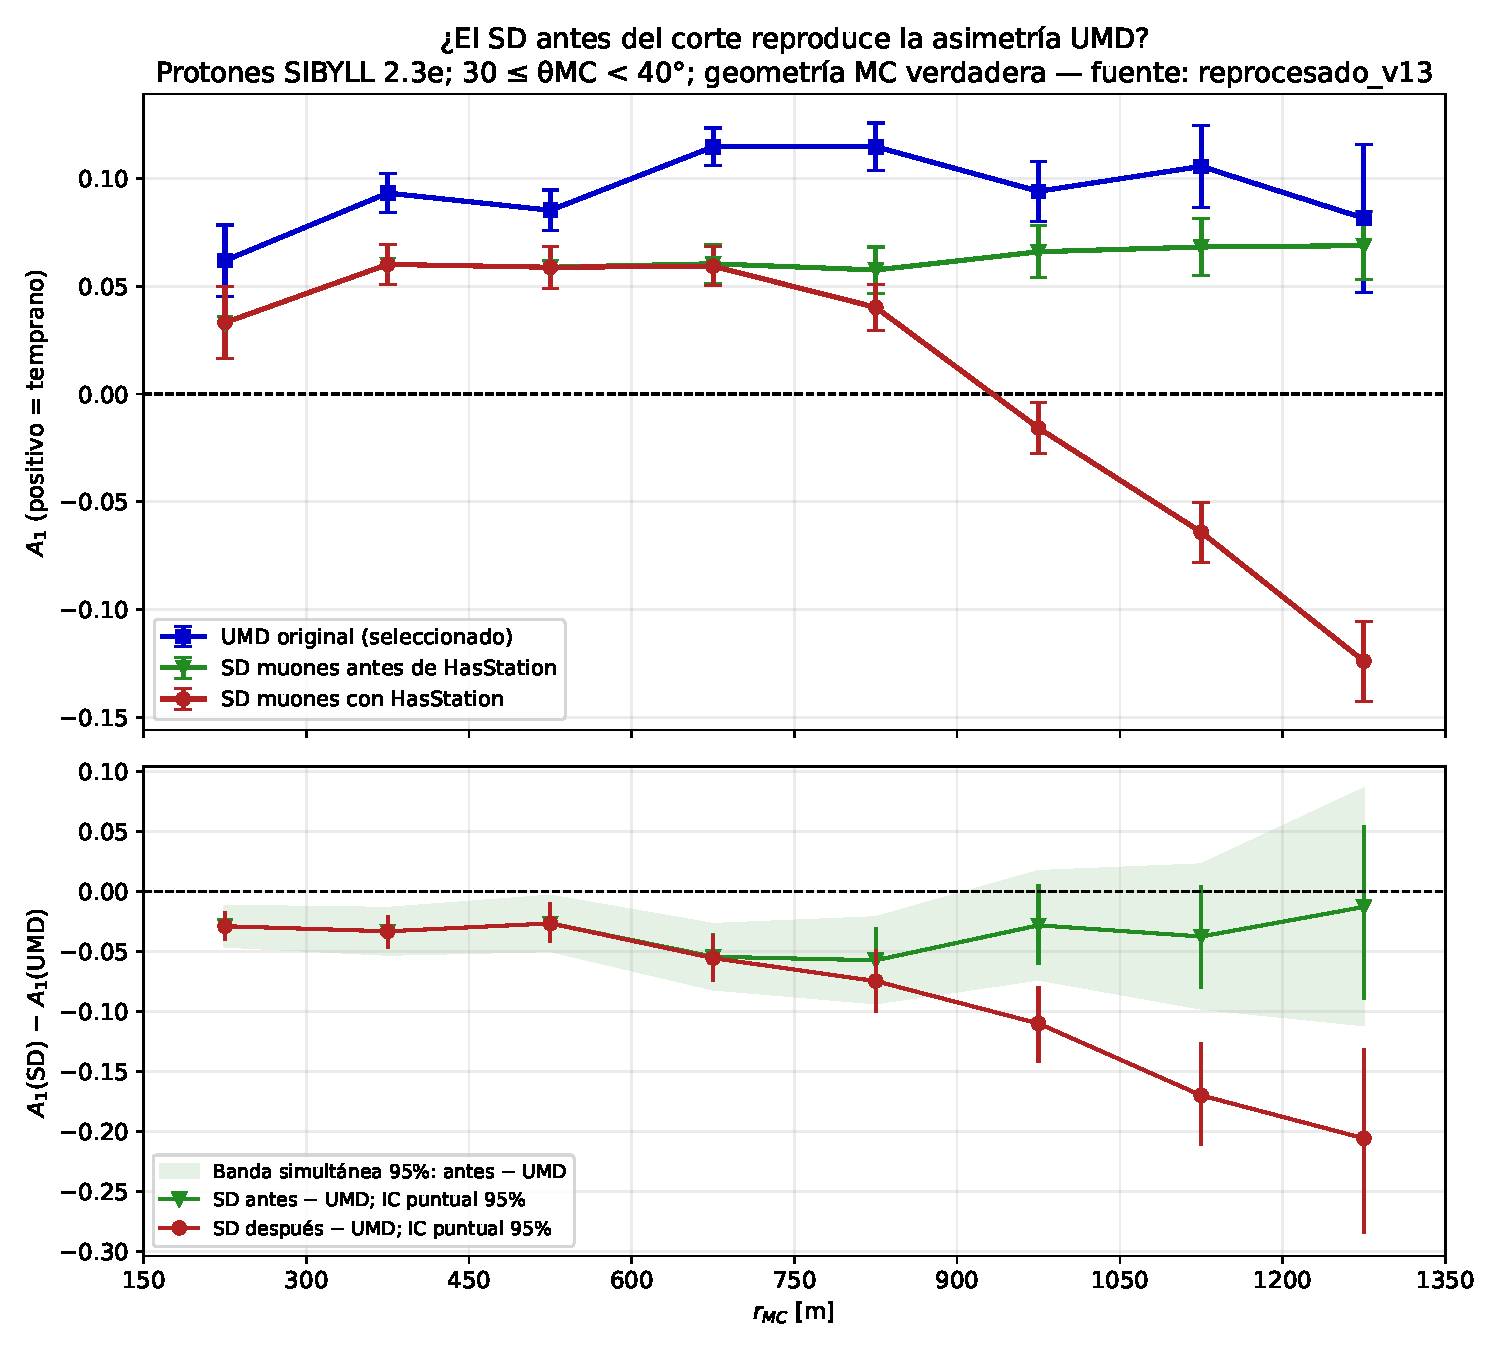
\includegraphics[width=0.72\linewidth]{SD_sin_corte_vs_UMD_reprocesado_v13.pdf}
  \caption{Resolución. Arriba: $A_1$ del UMD (azul, con su selección original), del SD muónico sin el
  requisito de estación reconstruida (verde) y con él (rojo), sobre los datos reprocesados. Abajo:
  diferencias SD$-$UMD con intervalos del 95\,\%. Persiste una diferencia menor por debajo de 900\,m, todavía
  sin explicar. Figura de \code{claude\_work/reprocesamiento\_sd\_completo/} (\code{c332ab8}), reutilizada.}
  \label{fig:resolucion}
\end{figure}

%=====================================================================
\section{Los flujos de trabajo}
%=====================================================================
\begin{figure}[t]
  \centering
  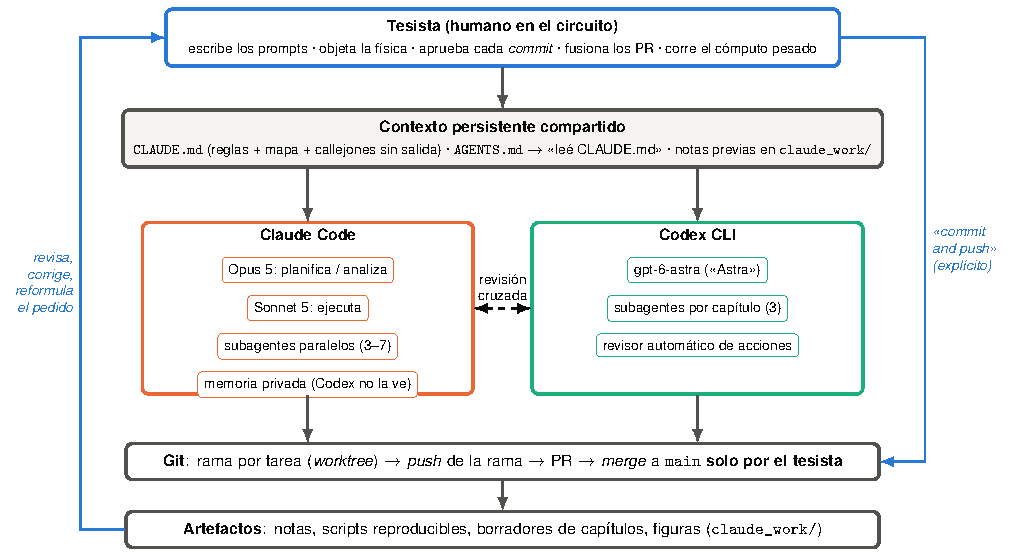
\includegraphics[width=\linewidth]{workflow.pdf}
  \caption{Flujo de trabajo observado. Ambos agentes leen \code{CLAUDE.md}; la memoria de Claude es privada.
  El tesista conserva los controles de \emph{commit}, fusión y cómputo pesado.}
  \label{fig:workflow}
\end{figure}

\paragraph{Memoria de proyecto.} \code{CLAUDE.md} funcionó como un cuaderno de reglas que crecía con cada
incidente: pedir permiso antes de \code{git}, nunca subir cambios (\emph{push}) a \code{main}, no dejar de
versionar los cuadernos. Cada regla nació de un error concreto y quedó en un \emph{commit} con su motivo.
Codex la heredó con un archivo de cinco líneas, \code{AGENTS.md}: «leé \code{CLAUDE.md} completo y seguilo».
Algunas reglas y lecciones de física quedaron sólo en la memoria privada de Claude, así que Codex no las vio.
Además, \code{CLAUDE.md} no se actualizó después del hallazgo y sigue explicando la inversión con muones
blandos.

\paragraph{Prompts.} El tesista usó consignas estructuradas:
\begin{itemize}
  \item un rol de árbitro de revista (EPJC);
  \item un orden de lectura y una regla de bibliografía;
  \item preguntas numeradas;
  \item «discutí conmigo si hace falta».
\end{itemize}
Varios prompts los reescribió o redactó un agente. Eso aportó estructura, pero también introdujo sesgos: una
reescritura agregó «tratá las notas GAP como más autorizadas», y el prompt para Codex promovió un resultado
negativo a «establecido».

\paragraph{Subagentes y paralelismo.} Se usaron para:
\begin{itemize}
  \item explorar el repositorio (tres, al crear \code{CLAUDE.md});
  \item leer literatura y auditar el código en paralelo (7/09);
  \item revisar con un agente adversarial (11/09);
  \item redactar capítulos, uno por agente, con un integrador (Codex, 24/09).
\end{itemize}

\paragraph{Revisión entre modelos y entre sesiones.} Hubo corrección entre sesiones del mismo proveedor
(Opus corrigió a Sonnet dos veces) y revisión entre proveedores, en ambas direcciones. Ninguno de los
\emph{commits} de Codex lleva firma de coautoría, así que en \code{git log} aparecen como trabajo propio del
tesista. Los de Claude sí la llevan (16 de Sonnet~5 y 12 de Opus~5).

\paragraph{Controles humanos.} Ningún \emph{commit} se hizo sin orden explícita, salvo el primero: el
\code{CLAUDE.md} inicial, que además se subió sin pedirlo. El 31/08 se hicieron sin confirmación específica
un \emph{force-push} y el borrado forzado de una rama. El tesista fusionó los 23 \emph{pull requests} y corrió
los trabajos pesados en el servidor compartido. En Codex, desde el 11/09 el tesista delegó las aprobaciones en
un revisor automático, para evitar confirmar cada comando a mano; siguió leyendo lo producido. Ese revisor emitió 109 veredictos, todos favorables, incluido el de la edición que
perdió 63\,747 filas. Evalúa riesgos operativos, no corrección.

%=====================================================================
\section{Qué funcionó y qué no}
%=====================================================================
{\small
\begin{longtable}{>{\raggedright}p{3.6cm}>{\raggedright}p{7.2cm}>{\raggedright\arraybackslash}p{3.8cm}}
\caption{Fallas observadas y quién las detectó.}\label{tab:fallas}\\
\toprule
\textbf{Falla} & \textbf{Episodio} & \textbf{Quién la detectó}\\
\midrule\endhead
Test que no puede fallar & El \emph{bootstrap} de filas «descarta» la selección (7/09, Claude) & Astra, 3 días después\\
Resumen con pérdida; autoridad heredada & El informe omite \code{HasStation}; el prompt lo da por «establecido» & Astra\\
Verificación que no lo era & Un chequeo numérico imprime \code{agreement: NO} y se informa como «verificado» (2/09, Claude) & Nadie, hasta este estudio\\
Paso del proceso inventado & Se redacta una «revisión adversarial» antes de lanzar el agente adversarial (11/09, Claude) & El propio agente, 8\,s después; no se lo informó al tesista\\
Lectura obligatoria salteada & Informe que declara novedades sin haber leído el trabajo previo indicado (7/09, Claude) & El tesista\\
Física incorrecta aceptada & Promedio de cocientes (Claude); resultado del SD trasladado al UMD (Claude) & El tesista\\
Método sobredimensionado & «Tu pipeline sin esa línea» era otro lector (Astra) & El tesista, preguntando\\
Código presentado sin ejecutar & Dos lectores listos «para correr» cuyas pruebas sintéticas aceptaban la pérdida de filas (Astra) & El tesista, al correrlo\\
Cambio de código silencioso & \code{or not simCounter}: $-63\,747$ filas, «inofensivo» (Astra) & El tesista, por el conteo de filas\\
Acción destructiva con garantía falsa & \code{git rm --cached} borró los cuadernos (y sus figuras) del tesista (Claude) & El tesista, al perder datos; recuperado\\
Acciones de \code{git} sin permiso & Primer \emph{push} sin pedirlo; \emph{force-push} y borrado de rama (Claude) & Nadie en el momento\\
Contexto desactualizado & \code{CLAUDE.md} sigue explicando la inversión con muones blandos; la conclusión de la charla la llama «real y no trivial», en tensión con su diapositiva sobre \code{HasStation} & Este estudio\\
Volumen excesivo & Carpetas v1--v4; un \emph{commit} de 144 archivos (+168 mil líneas) (Astra) & El tesista («json que no significan nada para mí»)\\
\bottomrule
\end{longtable}
}

Lo que funcionó, en orden de impacto:
\begin{enumerate}[label=(\roman*)]
  \item la \textbf{lectura independiente por un segundo modelo}, que rescató la hipótesis correcta y luego
  encontró errores del primero (y viceversa);
  \item \textbf{reproducir antes de extender}: Astra reprodujo la figura del tesista antes de modificarla, y
  Claude validó su lector fila a fila;
  \item la \textbf{memoria de proyecto}, que acumula reglas y callejones sin salida;
  \item las \textbf{objeciones del tesista}, tanto físicas (dos errores de los agentes corregidos) como
  metodológicas («¿usaste literalmente mi código?»);
  \item \textbf{mantener humanos} la fusión de cambios y el cómputo pesado.
\end{enumerate}
Hubo también aciertos laterales. Claude detectó que las barras de error publicadas del SD eran optimistas en
un factor $\sim\sqrt{3}$, por filas repetidas, y evitó una subida accidental a \code{main} por una rama mal
configurada \ev{\code{c332ab8}; \code{f032527f}}.

Un patrón se repite en la tabla~\ref{tab:fallas}. Los errores de \emph{ingeniería} más graves los detectó el
tesista, por el conteo de filas o al perder archivos. El error de \emph{razonamiento} más grave lo había
señalado un subagente del mismo sistema, y lo rescató otro modelo. La autorrevisión atrapó los menores.

%=====================================================================
\section{La lección clave}
%=====================================================================
La historia intuitiva sería «los agentes persiguieron la física y finalmente otro agente encontró el bug». La
evidencia muestra algo más interesante:
\begin{enumerate}
  \item \textbf{El marco inicial fue humano y razonable.} El tesista tenía un pipeline validado durante meses,
  el efecto aparecía con dos geometrías y dos reconstrucciones, y los prompts pedían explicar física. Ya había
  vivido un caso de «física» que era un error de pipeline, pero esa lección no se transfirió a esta anomalía.
  El punto ciego no fue un corte en particular: fue no preguntarse \emph{qué población representaba} el
  observable del SD.
  \item \textbf{La fenomenología bien hecha dejó una pista.} Un modelo que parece reproducir el UMD y falla
  sólo en el SD sugiere mirar qué tiene de distinto el \emph{observable} del SD. Opus lo planteó el 4/09. El
  7/09, otra sesión, sin haber leído ese documento, llegó por su cuenta a la misma pregunta.
  \item \textbf{La hipótesis se generó y se descartó el mismo día} (7/09), por un test inadecuado y un
  resumen que perdió el mecanismo. Tres días después, un traspaso convirtió ese descarte en certeza.
  \item \textbf{La rescató una lectura independiente.} Otro modelo, con otro contexto, leyó el código y el
  argumento estadístico por sí mismo. Con un solo caso no podemos separar tres factores: el cambio de
  proveedor, el hecho de empezar con contexto limpio y el empujón que daba el propio prompt de Claude, que
  pedía buscar una «selección a nivel de detector».
\end{enumerate}
Hay además un matiz irónico. La curva de la tesis que toda la fenomenología intentaba explicar estaba, ella
misma, sesgada por la selección, y según el tesista también lo estaba el $-0.10$ publicado en GAP-2026-041,
calculado con el mismo pipeline.

¿Ayudaron o entorpecieron? \textbf{Las dos cosas.} Generaron la hipótesis dos veces, montaron el
contrafactual sobre datos crudos en horas y lo verificaron de forma cruzada. También la descartaron con un
test que no podía fallar, propagaron ese descarte y entregaron código que perdía datos. No podemos saber si
el tesista, solo, lo habría encontrado antes o después: el requisito llevaba unos diez meses sin ser
cuestionado.

%=====================================================================
\section{Relación con los contenidos del curso}
%=====================================================================
\begin{itemize}
  \item \textbf{Schwartz, «Vibe physics»} \cite{schwartz}.
  \begin{itemize}
    \item Describe una práctica que aquí se repitió en ambas direcciones: «hice que GPT revisara el trabajo
    de Claude y viceversa».
    \item Su advertencia «dice \emph{verificado} cuando no lo verificó» tiene aquí un ejemplo literal (2/09)
    y uno análogo (11/09).
    \item Su tesis de que lo que falta es el «gusto» (\emph{taste}) se confirma a medias. Las objeciones
    físicas decisivas fueron humanas, pero también lo fue el punto ciego inicial.
  \end{itemize}
  \item \textbf{Mishra-Sharma, «Long-running Claude»} \cite{mishra}.
  \begin{itemize}
    \item «Los enfoques fallidos son importantes: sin ellos, las sesiones sucesivas vuelven a intentar los
    mismos callejones sin salida». Es lo que hacen \code{CLAUDE.md} y las retractaciones documentadas.
    \item El trabajo autónomo depende de que el agente «tenga una manera de saber si está progresando». Aquí,
    el UMD actuó como un oráculo parcial que señaló que el problema estaba del lado del SD.
  \end{itemize}
  \item \textbf{OpenAI Academy (FERMIACC)} \cite{openai}: el exceso de 750\,GeV del LHC ilustra el costo de
  explicar una señal que no es física. Aquí el costo fue menor, pero la nota GAP-2026-041 ya estaba publicada.
  \item \textbf{Dodelson} \cite{dodelson}: el resultado de Astra se verificó con una reimplementación
  independiente del lector (Claude, mismos ADST), dos chequeos aritméticos cruzados y la corrida propia del
  tesista, y todavía no entró al texto de la tesis. El juicio experto sigue siendo el paso final.
\end{itemize}

%=====================================================================
\section{Recomendaciones}
%=====================================================================
\begin{enumerate}
  \item \textbf{Auditar la población antes que la física.} Si un efecto aparece en un detector y no en otro,
  hay que preguntar qué población representa cada observable: cortes, \emph{joins} y bucles entre la
  simulación cruda y el gráfico. Después hay que probarlo con datos que incluyan lo excluido.
  \item \textbf{Preguntar de cada test si podría haber fallado en caso de que la hipótesis fuera cierta.} Si
  no, no es evidencia.
  \item \textbf{Los traspasos transmiten dudas, no veredictos.} Un resultado negativo viaja con su test y su
  alcance, nunca como «establecido».
  \item \textbf{Buscar una lectura independiente} (otro modelo, o una sesión con contexto limpio) que revise
  las premisas, no sólo las conclusiones.
  \item \textbf{Verificación ejecutable:} comparaciones con \code{assert}. Un \code{agreement: NO} impreso
  debe bloquear la afirmación.
  \item \textbf{Vigilar invariantes de población}: contar filas antes y después de cada cambio de lector. Un
  dato faltante no es un cero.
  \item \textbf{Exigir que el código se ejecute} sobre datos reales antes de darlo por listo; las pruebas
  sintéticas no alcanzan.
  \item \textbf{Mantener actualizado el contexto compartido} y guardar las reglas en el archivo que leen
  todos los agentes, no sólo en la memoria privada de uno.
  \item \textbf{Un revisor automático de seguridad no es un revisor científico.}
  \item \textbf{Mantener humanas la fusión de cambios y el cómputo pesado} en infraestructura compartida.
  \item \textbf{Pedir pocos entregables legibles}, como un resumen de una página y un cuaderno reproducible,
  en lugar de paquetes voluminosos.
\end{enumerate}
Para esta tesis, la consecuencia inmediata es concreta: los lectores de datos reales aplican el mismo
requisito. Toda comparación SD--UMD del capítulo 7 estará condicionada por construcción a la presencia de la
estación SD, sin una muestra «sin corte» con la que compararla.

%=====================================================================
\section{La voz del tesista}
%=====================================================================
Esta sección resume, a partir de sus respuestas a un cuestionario, la experiencia del tesista (L.~Silva
Pizzi) en primera persona.

\begin{quote}
\textbf{Sobre el corte.} Nunca había pensado en ese requisito como una selección. Lo había puesto porque, si
el SD no dispara, el UMD no guarda datos, así que esas estaciones parecían inútiles. Tampoco me había dado
cuenta de que no había auditado el pipeline: lo daba por revisado. Los comentarios de las IA sobre este
punto fueron extremadamente perspicaces.

\textbf{Sobre cómo trabajé.} Casi todo lo hice con los agentes en la terminal. Antes sólo había usado Gemini
como chat. Usé Claude y Codex a propósito para contrastar modelos y empresas: quería ver cómo se comportaban
uno frente al otro, y Astra se presentaba como un modelo de punta. Puse la aprobación automática en Codex
sólo para no tener que confirmar cada comando. Leí casi todo lo que produjeron, siempre que fuera legible;
nada se aceptó sin que yo lo leyera y lo reprocesara. Algunos informes se me hicieron difíciles de leer.

\textbf{Sobre qué me convenció.} No me convenció el primer resultado de Astra, sino revisarlo en detalle
después de varias iteraciones en las que lo hizo más claro: cuadernos documentados y la reproducción exacta
de mi propia figura.

\textbf{Sobre el aprendizaje en los dos sentidos.} Yo corregí física de los agentes varias veces, pero ellos
también corrigieron la mía. Por ejemplo, me aclararon cómo contribuye la geometría del tanque (muones que
entran por arriba o por el costado, y la energía que depositan).

\textbf{Balance.} La IA ayudó al cien por ciento: sin ella no habría pensado en el requisito. Mi director se
sorprendió, lo encontró creíble y me pidió controles adicionales que todavía tengo pendientes.
\end{quote}

\noindent Dos respuestas matizan lo que muestran los registros. El tesista no recordaba haber visto la sección
del 7/09 que «descartó» la selección. Tampoco había advertido que el prompt que pegó en Codex daba ese
descarte por «establecido», aunque sí leyó el prompt. Ambas cosas son coherentes con la tesis central de este
informe: el error viajó dentro de documentos largos, sin que nadie lo marcara.

%=====================================================================
\section{Limitaciones}
%=====================================================================
\begin{itemize}
  \item \textbf{Fuentes incompletas.} El enlace compartido de la conversación de Codex no fue accesible
  (usamos su registro local); el razonamiento interno de Codex está cifrado en los registros; las
  conversaciones previas con Gemini (chat web) no se conservaron.
  \item \textbf{Un informe sobre IA escrito con IA.} La reconstrucción la hizo Claude, cuyas fallas y cuya
  competencia aparecen en el relato. Mitigamos este sesgo con evidencia por afirmación y dos verificaciones
  independientes, pero el sesgo puede ir en cualquier dirección.
  \item \textbf{Sesgo retrospectivo.} Juzgamos el test del 7/09 conociendo la respuesta. Sin embargo, su
  defecto se deduce de la definición del estimador, y Astra lo señaló sin conocerla.
  \item \textbf{Un solo caso.} No permite atribuir el rescate al cambio de proveedor ni generalizar
  proporciones de éxito entre modelos.
  \item \textbf{El tesista es sujeto y coautor} de este estudio. Su testimonio se recoge por separado, en la
  sección anterior.
  \item \textbf{Alcance del resultado físico.} Todo es Monte Carlo: 20 archivos, protones, SIBYLL~2.3e,
  $30$--$40^\circ$, $\log_{10}(E/\mathrm{eV})=17.5$--$18$. «Sin el requisito» significa todas las estaciones
  simuladas escritas en los ADST. El mecanismo es una hipótesis, el UMD no se puede «des-seleccionar» y queda
  una diferencia SD--UMD sin explicar por debajo de 900\,m.
\end{itemize}

%=====================================================================
\section{Conclusiones}
%=====================================================================
Los agentes aceleraron la mayoría de los pasos técnicos de esta investigación y produjeron la hipótesis
correcta dos veces. El obstáculo no fue la falta de ideas sino la validación: un test que no podía fallar,
una cadena de resúmenes que convirtió una duda en certeza y código que se dio por listo sin correrlo. Lo que
destrabó el problema fue una combinación que el curso anticipaba: una lectura independiente, reproducir antes
de extender y un humano atento a invariantes simples. La lección que nos llevamos es metodológica y vale
también sin IA: \emph{antes de explicar un efecto, hay que preguntarse qué hizo el análisis para que el efecto
exista.}

\appendix
\section{Cómo se produjo este informe}\label{ap:metodo}
% Apéndice A — cómo se produjo este informe (se incluye desde informe.tex)
Este informe se produjo con el mismo tipo de herramientas que analiza, y el proceso tuvo sus propias
fallas; las registramos por coherencia.

\paragraph{Organización.} Una sesión de Claude Code (Opus~5.5), aislada en una rama propia y sin permiso
para hacer \emph{commits} sin autorización explícita, actuó como coordinadora. Primero convirtió las
transcripciones locales (unos 60\,MB de JSONL) en texto legible (3\,MB) con un script propio, excluido
del control de versiones porque las transcripciones pueden contener rutas internas del servidor de la
colaboración. Luego escribió una consigna común (\code{notes/AGENT\_BRIEF.md}) con el estándar de
evidencia y una plantilla de notas, y lanzó ocho agentes de lectura en paralelo:
\begin{center}\small
\begin{tabular}{ll}
\toprule
Agente & Fuentes\\
\midrule
T1, T2, T3 & transcripciones de Claude (29/08--02/09, 03/09--10/09, 10/09--23/09)\\
C1, C2 & transcripciones de Codex (hilo principal de Astra; sesiones posteriores)\\
R & artefactos en \code{claude\_work/} (linaje de cada afirmación física)\\
G & \code{git}, \emph{pull requests}, \code{CLAUDE.md}, \code{AGENTS.md}, memoria, prompts\\
P & cuaderno de laboratorio, evolución de scripts, notas GAP y capítulos de la tesis\\
\bottomrule
\end{tabular}
\end{center}
Un noveno agente verificó contra las fuentes primarias 21 afirmaciones clave (20 confirmadas, 1 con
matices) y un décimo revisó el primer borrador en modo adversarial.

\paragraph{Fallas del propio proceso.}
\begin{itemize}
  \item \textbf{Nuestra consigna tenía el signo al revés.} El resumen inicial decía que \emph{quitar} el
  requisito producía la inversión; es al revés. Lo detectó el primer agente en terminar, contrastando con
  los números de las sesiones; corregimos la consigna y avisamos a los demás agentes en curso. Es el mismo
  tipo de error que estudia el informe: una afirmación del coordinador que, sin verificación, se habría
  propagado a todos los agentes.
  \item \textbf{Límite de uso.} Siete de los ocho agentes fueron interrumpidos por el límite de sesión de la
  cuenta; seis ya habían escrito sus notas completas y dos se relanzaron horas después con la instrucción
  de escribir la nota antes del resumen final.
  \item \textbf{Fricción de herramientas.} El aislamiento de la sesión rechazaba cualquier comando cuyo
  texto contuviera la cadena «git» (incluida la ruta \code{/Github/}); se resolvió con scripts auxiliares.
  \item \textbf{Una cita inventada por una herramienta.} El resumen automático de una página web nos atribuyó
  a Schwartz la frase «se atraparon errores mutuamente», que no figura en el artículo. La detectó el revisor
  adversarial y la eliminamos tras reverificar textualmente todas las citas del curso.
  \item \textbf{El primer borrador tenía errores de fondo.} La revisión adversarial (61 observaciones) encontró
  que el borrador atribuía el sesgo sólo a la línea \code{HasStation} (la selección estaba también en la
  estructura de los datos), omitía que todo es Monte Carlo y que el UMD también está seleccionado, recortaba
  una cita condicional, afirmaba una relación causal que la transcripción contradice y tenía tres conteos mal.
  Esta versión incorpora esas correcciones.
  \item \textbf{Fuente inaccesible.} El enlace compartido de ChatGPT devolvió un error de acceso; usamos el
  registro local de Codex; según el tesista todo el trabajo se hizo por terminal, así que es la misma
  conversación.
\end{itemize}


\section{Cronología detallada}\label{ap:crono}
% Apéndice B — cronología detallada (horas en UTC; hora local = UTC−3)
{\small
\begin{longtable}{>{\raggedright}p{2.3cm}>{\raggedright}p{2.2cm}p{7.2cm}>{\raggedright\arraybackslash}p{2.8cm}}
\toprule
\textbf{Fecha} & \textbf{Actor} & \textbf{Hecho} & \textbf{Evidencia}\\
\midrule\endhead
09/10/2025 & tesista & Aparece el chequeo \code{HasStation} (protección contra nulos) & \code{e9a2737}\\
04/11/2025 & tesista & Regla del cuaderno: cortes de calidad como banderas, filtrar después & \code{Trabajo.tex:168}\\
05--11/11/2025 & tesista & \code{HasStation} pasa a descartar la fila; rotulado «Corte de Calidad 1» & \code{41b98be}, \code{ce4e0eb}\\
13/07/2026 & tesista & Se abandona el Monte Carlo rápido para explicar la inversión & \code{6d6b97b}\\
28/08/2026 & curso & Clase «Primeros pasos con Claude Code» & cronograma\\
29/08 & Sonnet~5 + 3 subag. & Se crea \code{CLAUDE.md}; primera revisión de las notas GAP & \code{fa012d6}; \code{c468bc17}\\
31/08 & Opus~5 & Segunda revisión: corrige la primera & \code{df3c0277}\\
02/09 14:26 & tesista & «podríamos chequearlo después»: la inversión se da por física & \code{df3c0277}\\
02/09 15:03 & Sonnet~5 & Chequeo con \code{agreement: NO} informado como «verificado» & \code{df3c0277}\\
02/09 & Opus~5 / Sonnet~5 & \code{git rm --cached}: se pierden los cuadernos del tesista; recuperados & \code{40e7257}, \code{77ad431}\\
04/09 05:00 & tesista $\to$ Opus~5 & Corrección espectral: UMD $+0.13$/$+0.11$, SD $+0.19$/$-0.10$ & \code{67ae9e4}\\
07/09 14:12 & subagente Opus~5 & Señala \code{HasStation} como compuerta de selección & \code{a7da6dcd}\\
07/09 14:23 & Sonnet~5 & «no sobrevive a la prueba directa» (\emph{bootstrap} de filas) & \code{60fca507}\\
10/09 13:41 & tesista & «B\&B es del SD»: retractación y memoria permanente & \code{88fffbb}\\
10/09 14:06 & Sonnet~5 & Redacta el prompt para Codex («tratar como establecido») & \code{60fca507}\\
10/09 14:22 & Astra & «Eso no queda descartado por el bootstrap anterior» & Codex \code{01a08ba1}\\
10/09 19:30 & Astra & 20 archivos: $+0.068\to-0.095$, IC\,95\,\% de la diferencia $[-0.178,-0.145]$ & Codex \code{01a08ba1}\\
11/09 03:16 & Astra & Reproduce la figura del tesista; $+0.069\to-0.124$ (1200--1350\,m) & \code{02\_reproduccion}\\
11/09 08:18 loc. & Astra & \emph{Commits} del paquete y del resumen para el director & \code{b072c09}, \code{98a48c9}\\
11/09 17:10 & Opus~5 / Sonnet~5 + 6+1 subag. & Revisión escéptica de Astra: «parcialmente de acuerdo» & \code{REVIEW\_ASTRA}\\
17/09 13:49 & tesista & Nota la pérdida de filas del lector de Astra & Codex \code{01a08ba1}\\
17/09 & Opus~5 & Lector de dos tablas; el tesista corre el reprocesamiento & \code{8d4b5a0}, \code{0ecae20}\\
17/09 & tesista & Charla RAFA 2026, con el resultado como «análisis preliminar» & \code{114fd52}, \code{ca3037a}\\
23/09 23:44 & Astra & Audita el reprocesamiento de Claude; tres huecos de validación & Codex \code{01a08ba1}\\
24/09 00:17 loc. & Opus~5 & Confirmación sobre el pipeline del tesista & \code{c332ab8}\\
24/09 03:24 & Astra + 3 subag. & Borradores de los capítulos 3, 5 y 6 & \code{borradores\_\ldots}\\
\bottomrule
\end{longtable}
}


\begin{thebibliography}{9}
\bibitem{schwartz} M.~Schwartz, «Vibe physics: The AI grad student», Anthropic Science Blog (2026).
\bibitem{mishra} S.~Mishra-Sharma, «Long-running Claude for scientific computing», Anthropic Science Blog (2026).
\bibitem{openai} OpenAI Academy, «How Physicists Are Using AI to Chase New Physics» (2026).
\bibitem{dodelson} S.~Dodelson, «Evolving Dark Energy and AI», Substack (2026).
\bibitem{gap041} GAP-2026-041, nota interna de la Colaboración Pierre Auger (2026).
\bibitem{bb} X.~Bertou y P.~Billoir, GAP-2000-017, nota interna de la Colaboración Pierre Auger (2000).
\bibitem{cazon} L.~Cazón \emph{et al.}, «A model for the transport of muons in extensive air showers», Astropart.\ Phys.\ 36 (2012) 211--223.
\end{thebibliography}
\end{document}
